\section{Preliminary Need-Finding}
\subsection{LLM Baseline}

With the purpose of gathering valuable information in an efficient way, maintaining an open mind-set not to be occluded by our initial ideas, we needed to formulate questions specific on what we were interested in.\\
Therefore, we first came up with a set of topics and then decided to use an LLM (Large Language Model) to get a preliminary list of possible questions for each of them.




As result of our prompt Fig \ref{fig_prompt} ChatGPT proposed a list of questions we used as a starting point. The questions were too many and sometimes repetitive, so we had to reformulate many of them and reduce redundancies.\\
\begin{figure}[ht]
    \centering
    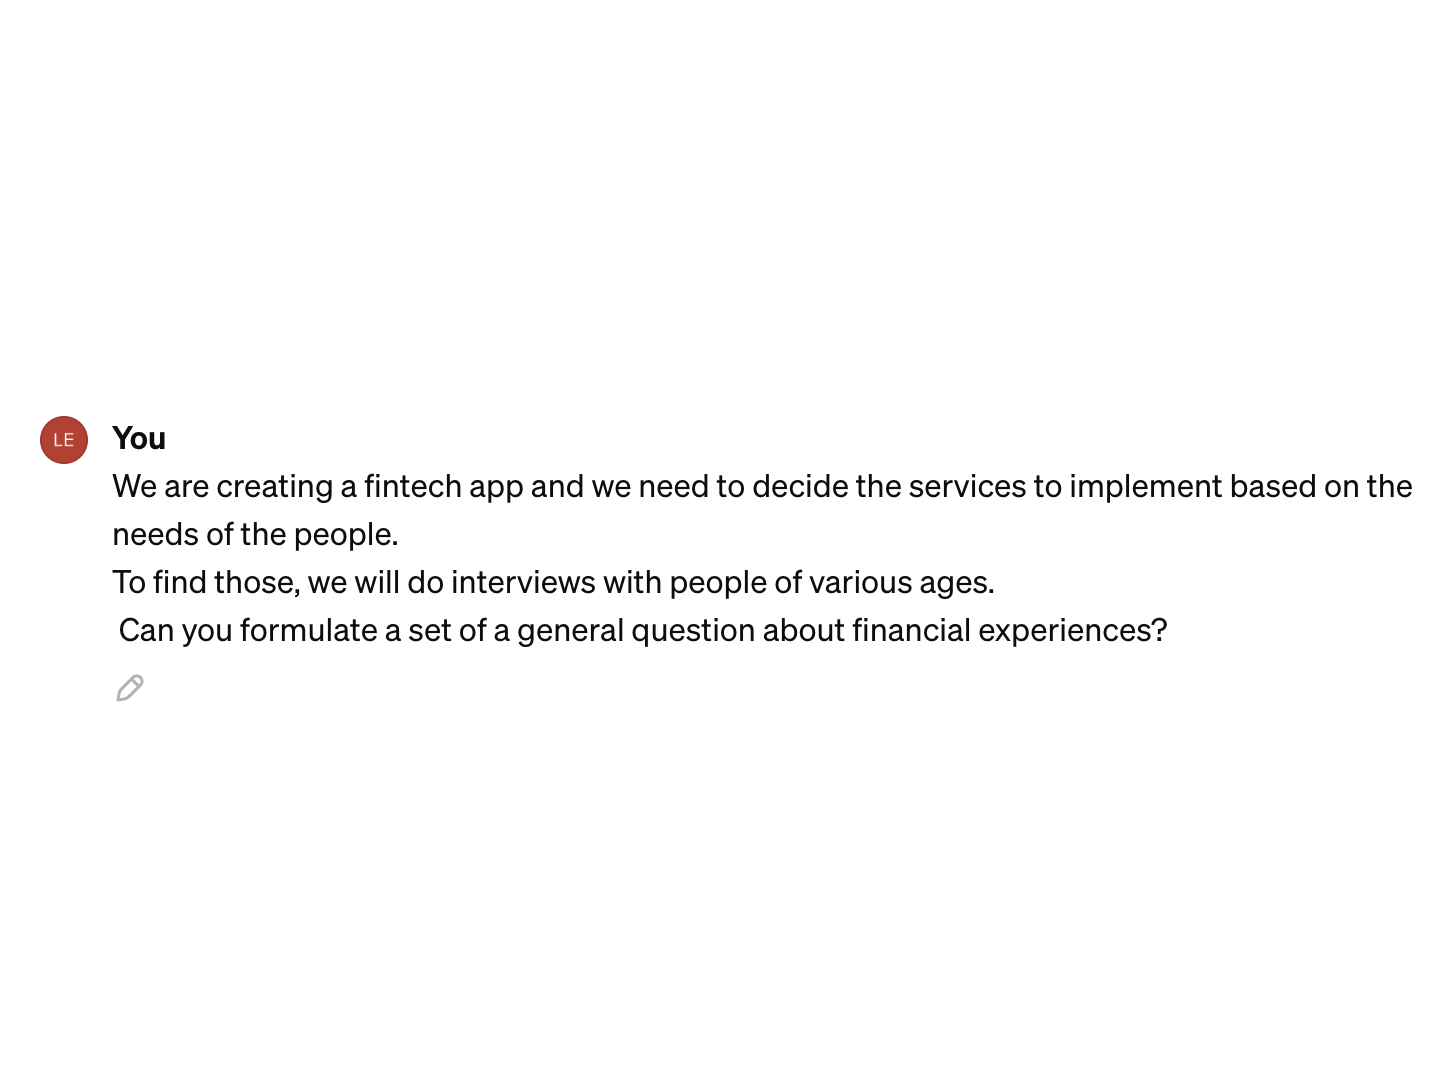
\includegraphics[width=0.5\linewidth]{figures/prompt.png}
    \caption{ChatGPT prompt}
    \label{fig_prompt}
\end{figure}

\subsection{First Interviews}
With questions we considered ready, we approached our first candidate; the result of this first interview taught us two things. First, some questions were obvious or not able to produce useful information; second, they were too many, and contrarily to what expected, the interview lasted about 10 minutes.\\
Fortunately, the interviewee kindly gave us feedback, which was deeply appreciated. We thus needed to further refine and reduce the number of questions, but still ensuring to cover all the macro fields and provide the candidates room to share their experiences.\\
We therefore decided, after refining our questions(available at this \href{https://docs.google.com/document/d/1L25VnXD9_-V7enQ3jEuFU-7WAiuKRug0KEyd9jIrUYU/edit?usp=sharing}{\textbf{link}}), not to propose the whole set of questions to every candidate, but to partition them in batches and ask interviewees only a few of them. In this way, we did not restrict our possibilities of gaining data, and at the same time we reduced the busy time per subject to about 3 minutes.\\
We also opted for asking our chosen LLM also to generate virtual personas and produce answers putting itself in their shoes. LLM's are trained on a big amount of real data, therefore, conceptually, they should be able to represent the average individual for each persona. As expected, it was able to provide reasonable opinions, nevertheless, we still had to gather information from real subjects in order to get a verification or a contradiction.
\subsection{Preliminary Questions Data Analysis}
We had to choose a specific fintech aspect to continue the design process with and the interviews significantly helped us in taking the right decision.\\
We were able to perform in total 20 interviews, and to get a general idea on what people think regarding the proposed topics, we interviewed people around La Sapienza, trying to keep the group as heterogeneous as possible in age, sex, nationality, profession, field of study, place and time.
Some observations from the most recurring responses are the following:\\
Concerning shared expenses, there's a preference for apps like Splitwise or Tricount despite some initial difficulties in using them. It’s not rare to use notes (physical or digital) to keep track of expenses, but this is defined as a suboptimal method, with frequent confusion and mismatch in records; the same problems are encountered when only chat services are used to coordinate.\\
The most utilised payment method is the credit card. Many have successfully experimented with online payments (e.g. PayPal), although some needed to be more intuitive. \\
Lastly, a few practice investing in stocks or cryptocurrencies, utilising specific platforms with benefits and drawbacks. The other interviewees prefer to refrain from investing due to a lack of knowledge or trust.\\
Most are interested in deepening their financial knowledge, and they consider online courses a good resource for this purpose at the expense of face-to-face lessons.
With this information we could discard some of the proposed topics and make some interesting observations on others.
First of all, we excluded investments, cryptocurrencies, blockchain and loans because most people do not know very much on these topics and the few which gave us a positive answer said to already have all the tools needed. Furthermore, we neither have a solid basis to start from, so we did not have enough information to design a relative application.\\
We excluded also cybersecurity, this because interviews did not gave us any evident problem whose solution was suitable for this project.\\
The remaining topics were payments and transactions, personal and shared expenses.
Regarding the first there exist already many affirmed applications which already do this like Paypal or Satispay and we thought that creating a competitor would have been redundant.
Nevertheless, we singled out from multiple interviewees some common problems regarding the management of personal and shared finances:
\begin{itemize}
    \item Lack of awareness in expenses.
    \item Difficulty, also with already existent applications to clearly keep track of a shared fund, and relative problems related to this issue.
\end{itemize}
This gave us a strong clue on a need many people could have, we therefore decided to continue with this track.
\subsection{Study of Competitor Apps}
We studies this, this and this and the problem we found were...\\
After interviews and this study we had a more clear idea on what problems are.
\section{Need Finding on the Specific Topic}
\subsection{Survey on financial habits}
Having this first fairly realistic basis to start with, we could proceed to the next step.
We formulated 
\subsection{Interviews on Financial Habits}
The interviews shed light on various approaches to personal finance management and shared expenses. Most interviewees track their daily expenditures, mostly with banking apps or notes. While the first method is said to reliable, especially when tracking small expenses, the notes method is considered less organised. Others opt not to do so, but some would like to begin.

It was possible to note how the answers given by ChatGPT at the beginning of our need finding process were absolutely not far from the ones given by the interviewed persons, consolidating our assumption in considering both the real and digital personas' answers as reliable.

Based on the responses, we focused on two specific subtopics: tracking expenses and managing shared funds. With these concepts in mind, we developed a questionnaire to reach a broad audience quickly while working on other tasks. To see the questionnaire follow this \href{https://docs.google.com/forms/d/e/1FAIpQLScUr2eKVN_sTKEUXZMMJ9fErrNDnPoO3Dy4FSIO6jOAXINm9Q/viewform}{\textbf{link}}.

\begin{figure}[ht]
     \centering
     \begin{subfigure}[b]{0.45\textwidth}
         \centering
         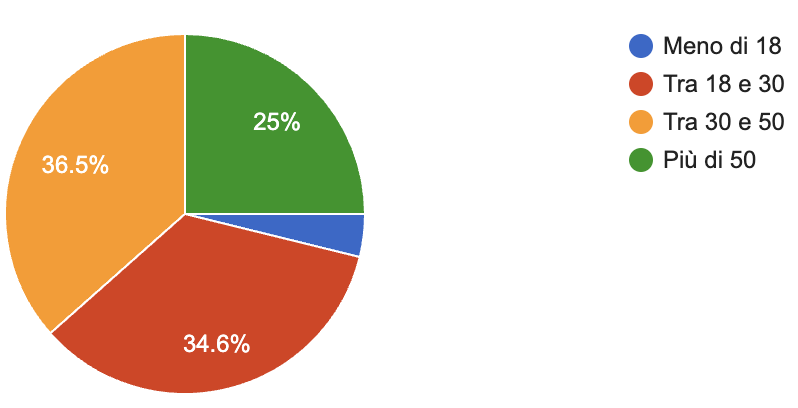
\includegraphics[width=\textwidth]{figures/sexes.png}
         \caption{Age covered}
         \label{fig_age}
     \end{subfigure}
     \hfill
     \begin{subfigure}[b]{0.45\textwidth}
         \centering
         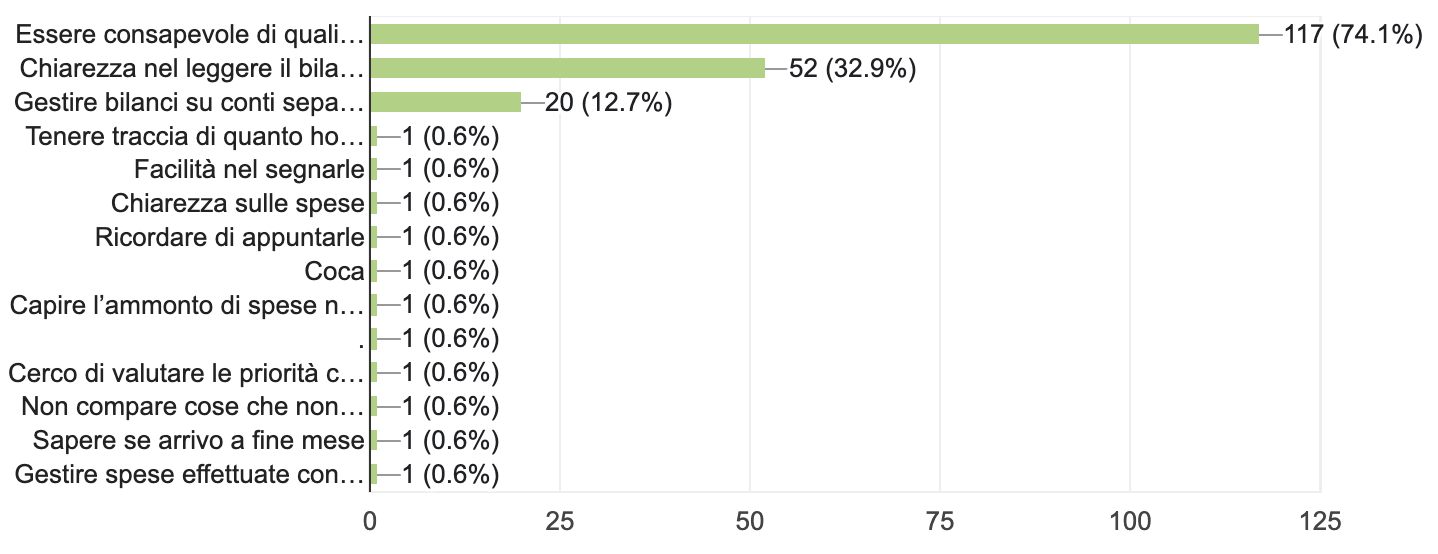
\includegraphics[width=\textwidth]{figures/needs.png}
         \caption{Needs}
         \label{fig_needs}
     \end{subfigure}
        \caption{Age covered (a) and needs (b) were two of the most interesting results}
        \label{fig_results_quest}
\end{figure}

\subsection{Deepening people's needs and features individuation}
The data gleaned from the questionnaire were highly informative and corroborated the needs we initially identified during the first interviews. The participant demographics showed a balanced age distribution Fig.\ref{fig_age}, and importantly, the primary needs expressed in the questionnaire results mirrored those we recognised at the outset Fig.\ref{fig_needs}.$\\$
Despite having initial areas of focus where we would have looked to find the task, we did a second round of interviews based on the questionnaire results. This was to ensure that the needs we identified were truly relevant, so we focused on asking people about their preferences for features involved in money-saver applications. We asked people more specific questions about managing personal and shared finances to understand people's needs.$\\$
Most interviewees stated their need to manage group finances and expenses, evidencing their difficulties. The main problem is the organisation: people lack coordination, causing problems understanding each one’s responsibility for the shared budget or expenses. The availability of a digital service is said to be a possible way to mitigate these situations.
Among the proposed features, two were particularly well-received, sparking inspiration and motivation within our team:$\\$
- Creating a shared fund to prepare a future collective expense, with a step-by-step guide on how and when to collect each personal share.$\\$
- the visualisation of expense records and history$\\$
While the presence of an in-app chat service is redundant, given all the similar services already used, the possibility of in-app payments is considered a good feature, with a little presence of distrust in connecting the personal bank fund/credit card.